\chapter{Le système masse-ressort}
Le système masse-ressort constitue en une masse suspendue à un ressort. Il peut aussi s'agir d'une masse posée sur une surface plane et reliée à un ressort. Il n'y a pas de frottements entre la masse et la surface plane.

\begin{figure}[ht!]
    \begin{minipage}{.5\textwidth}
        \centering
        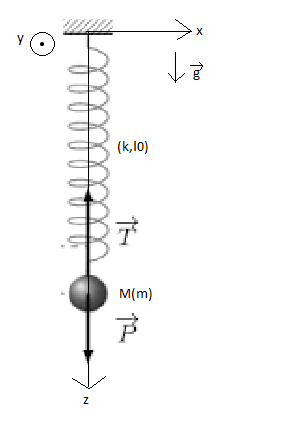
\includegraphics[width=.8 \linewidth]{masse_ressort_I.png}
        \caption{Système masse ressort.}
        \label{masse_ressort_I}
    \end{minipage}
    \begin{minipage}{.5\textwidth}
        \centering
        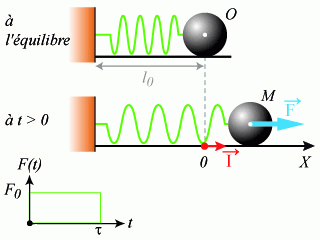
\includegraphics[width=.8 \linewidth]{bloc_ressort_I.png}
        \caption{Système bloc-ressort horizontal.}
        \label{bloc_ressort_I}
    \end{minipage}
\end{figure}

\newpage

Si la masse est déplacée vers la gauche par rapport à sa position d'équilibre, le ressort exerce une force opposée  et proportionnelle au déplacement. Une telle situation correspond aux conditions du MSH.
Dans le système masse ressort, la constante de proportionnalité liant l'élongation à la force de rappel est la constante de raideur du ressort. Puisque \(k=m \cdot \omega ^2\) alors :

\begin{equation}
    \tcboxmath[colback=LightBlue,colframe=blue]
    {\omega = \sqrt{\frac{k}{m}}}
\end{equation}


Si on se rappelle que \(\omega=2 \cdot \pi \cdot f\), on déduit que :

\begin{equation}
    \tcboxmath[colback=LightBlue,colframe=blue]
    {f=\frac{1}{2\pi} \cdot \sqrt{\frac{k}{m}}}
\end{equation}

\newpage

\section{Exercices}
\begin{exercise}
    Un oscillateur effectue 20 allers-retours en \(5,64 secondes\). L'objet en oscillation a une masse de \(145g\). Calcule la constante de raideur du ressort.
\end{exercise}

\begin{exercise}
    Il faut une force de 0,064N pour étirer de 4cm un ressort de sa position d'équilibre. On y attache un objet dont la masse est de 200g et on laisse osciller le tout librement. Calcule la période et la fréquence du mouvement.
\end{exercise}

\begin{exercise}
    Un objet d'une masse de 500[g] est attaché à un ressort. Le graphique ci-dessous représente son élongation au cours du temps.
    \begin{enumerate}[a)]
        \item Calcule la constante de raideur du ressort.
        \item Calcule l'intensité de la force résultante agissant sur l'objet lorsque l'élongation est maximale.
    \end{enumerate}
    \begin{figure}[ht!]
        \centering
        \begin{tikzpicture}[scale=0.75]
            \tikzset{>=latex}
            \tkzInit[xmin=0,xmax=1,ymin=-10,ymax=10,xstep=0.1,ystep=2]
            \tkzGrid
            \tkzDrawX[label={$t [s]$},below left=25pt]
            \tkzDrawY[label={$Y [mm]$},right=5pt]
            \tkzAxeXY[label={}] %This macro combines the four macros: \tkzDrawX\tkzDrawY \tkzLabelX\tkzLabelYnode font=\tiny]
            \tkzFct[domain=0:1,red]{8*sin(0.5*pi*x)}
        \end{tikzpicture}
    \end{figure}
\end{exercise}

\begin{exercise}
    \begin{minipage}[t]{0.4\textwidth}
        \qrcode{https://www.vf-bxl-moodle.be/mod/quiz/view.php?id=1369}
    \end{minipage}
\end{exercise}
